\documentclass[10pt, xcolor=table, dvipsnames]{beamer}
\usepackage[scale=3]{beamerposter}
\setlength{\paperwidth}{72in} % A0 width: 46.8in
\setlength{\textwidth}{72in}
\setlength{\paperheight}{45 in} % A0 height: 33.1in
\setlength{\textwidth}{45 in}
\usepackage[overlay,absolute]{textpos}
\usepackage{tikz}
\usetikzlibrary{shapes,arrows, fit}
\usepackage{tcolorbox}
\tcbuselibrary{raster}
\usepackage{enumitem}
\setlist{label=\textbullet} 
\usepackage{multicol}
\usepackage{multirow}
\usepackage{booktabs}
\usepackage{longtable}
\usepackage{array}
\usepackage{multirow}
\usepackage{wrapfig}
\usepackage{float}
\usepackage{colortbl}
\usepackage{pdflscape}
\usepackage{tabu}
\usepackage{threeparttable}
\usepackage{threeparttablex}
\usepackage[normalem]{ulem}
\usepackage{makecell}
\usepackage{xcolor}
\TPGrid[20mm,20mm]{1}{1}
\tcbset{%
	noparskip,
	colback=white, %background color of the box
	colframe=black, %color of frame and title background
	coltext=black, %color of body text
	coltitle=black, %color of title text 
	colbacktitle=Violet!30,
	boxrule=4pt,
	fonttitle=\bfseries,
}
\usepackage{xcolor}
\usepackage{soul}
\makeatletter
\let\HL\hl
\renewcommand\hl{%
	\let\set@color\beamerorig@set@color
	\let\reset@color\beamerorig@reset@color
	\HL}
\makeatother
\usepackage{pifont}
\newcommand{\cmark}{{\color{ForestGreen}\ding{51}}}
\newcommand{\xmark}{{\color{red}\ding{55}}}%
\newcommand{\qmark}{{\color{blue}\textbf{?}}}%
\begin{document}
	\begin{textblock}{1}(0.0,0)
		\begin{tcolorbox}[colback=Violet!30]{}
			
			
			\begin{centering} 
				\bigskip
				
				{\LARGE\textbf{Communicative reduction in referring expressions \\ within a
						multi-player negotiation game}}\\
				{\Large Veronica Boyce, Michael C. Frank} \\
				{Stanford University, send correspondence to vboyce@mit.edu}	
				
			\end{centering}
		\end{tcolorbox}
	\end{textblock}
	
	\begin{textblock}{.32}(0,0.16)
		\begin{tcolorbox}[title= {\centering Goals }]
			\begin{small}\centering
				\bigskip
			The ability to form novel conventions is a key signature of efficient
			linguistic communication.
 In dyadic reference games, we commonly observe 
 \begin{itemize}
 	\item \textbf{reduction} as utterances shorter over time,
 	 \item \textbf{convergence} within groups to a shared nick name,
 	  \item \textbf{divergence} between groups as each focuses on different features.
   \end{itemize}  CITATIONS

Do these phenomena occur in strategic games with more complex goals?


			\end{small}
		\end{tcolorbox}
	\end{textblock}
	
	

	\begin{textblock}{.32}[0,1](0,1 )
		\begin{tcolorbox}[title={\centering Experimental design }]

			
			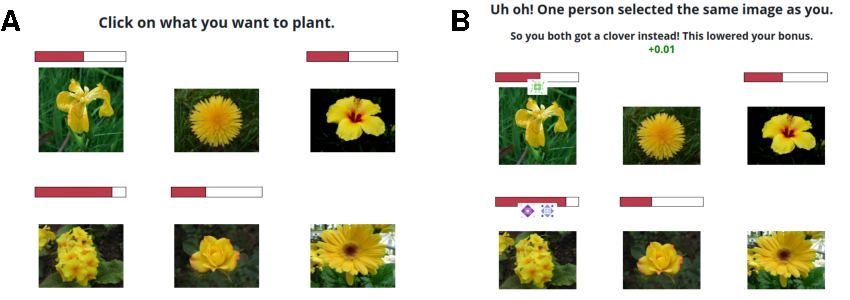
\includegraphics[clip,width=\textwidth]{interface-1.pdf}
			
			\begin{small}
				 During selection (A) each participant sees 6 flowers, 4 with value bars. Players can use a chat box to communicate before making selections. Then they see feedback (B) indicating who chose what.  When multiple players select the same flower, they recieve a lower value rather than what is shown. 

				In \emph{individual utility} games (18 games), each player earned points for the
				flowers they selected; in the \emph{shared utility} games (21 games), the points
				were averaged together, and all players in a game got the same reward.
								Each group plays 24 trials with images drawn from a set of 12 flowers. This data was first presented in  Mankewitz et al. (2021).
								
								We measure distance between two utterances by the cosine of the angle between their embedings using SBERT (CITATION). 
								
								
			\end{small}
		
		\end{tcolorbox}
	\end{textblock}
	
	
	\begin{textblock}{.41}[0,0](.33,.16)
	\begin{tcolorbox}[title={\centering Referring expressions reduce over time}]  
		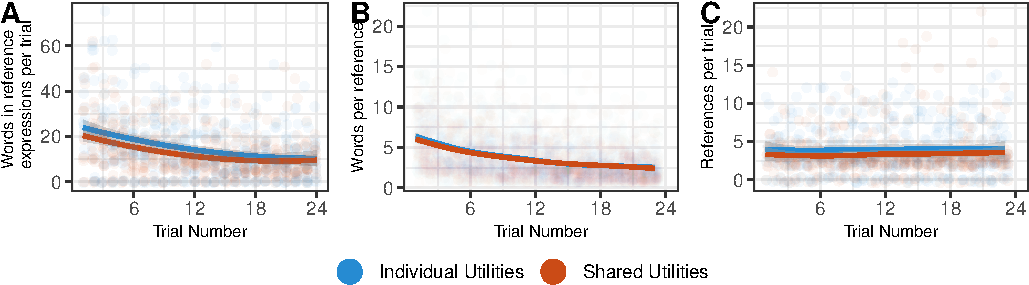
\includegraphics[width=.95\textwidth]{wordcount-1.pdf}    
		
	\begin{small}	Over time individual utterances shorten, but the same number of referring expressions are produced.     \end{small}                                              
	\end{tcolorbox}
\end{textblock}

	
		\begin{textblock}{.41}[0,0](.33,.43)

		\begin{tcolorbox}[title={\centering Expressions converge within groups}]  
			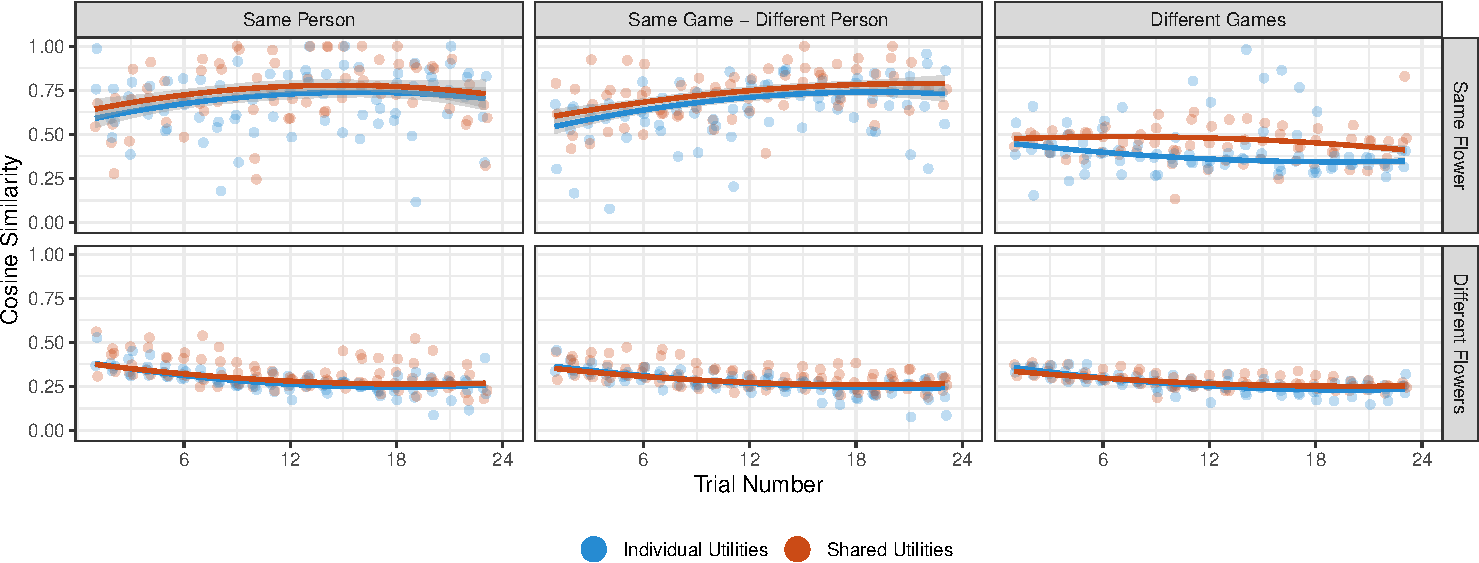
\includegraphics[width=.95\textwidth]{during-1.pdf}                            			                                                  
			\begin{small}
				
				Descriptions to the same flower in nearby trials increase in similarity with a group. 
				
				Similarity decreases slightly for the same flower across games. 
				
				Flower names become more distinctive as descriptions for two different flowers become less similar. 
				
			\end{small}
		\end{tcolorbox}
	\end{textblock}


	\begin{textblock}{.41}[0,1](.33,1)
	\begin{tcolorbox}[title={ \centering 					Incentive conditions differed a bit}]  
		\begin{minipage}{.45\textwidth}
			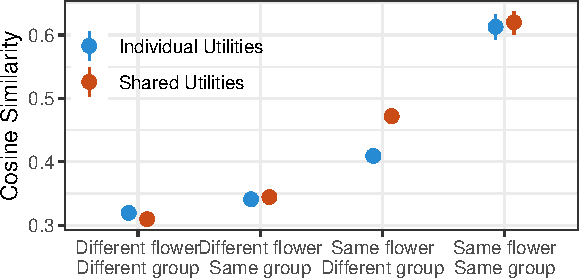
\includegraphics[width=\textwidth]{withinend-1.pdf}    
		\end{minipage}
	\hfill
	\noindent
	\begin{minipage}{.45\textwidth}
				\begin{small}
					
				Individual and shared utilities conditions differed slightly in divergence rate during games (above). In post-game descriptions (left), shared utility games show greater cross-game similarity for the same flowers than individual utility.
				
				\end{small}
	\end{minipage}

		
		                        			                                                  
	\end{tcolorbox}
\end{textblock}


		\begin{textblock}{.25}[1,0](1,.16)
	\begin{tcolorbox}[title={\centering Examples}]
		
		\centering
		\begin{footnotesize}
			Descriptions of different flowers from different games, illustrating reduction and convergence phenomenon. Images from experimental design: flower 1 upper left, flower 2 lower center, flower 3 lower left.
			\vspace{-1em}
			
			\centering
			\begin{tabular}[t]{llr>{\raggedright\arraybackslash}p{16em}}
				\toprule
				Flower & Game & Trial & Expression\\
				\midrule
				1 & 1A & 2 & not sure what kind of flower it is but the droopy-ish one\\
				1 & 1C & 4 & droopy iris flower\\
				1 & 1B & 21 & droopy\\
				\midrule
				2 & 2B & 2 & the red middle with spike\\
				2 & 2B & 3 & the red center\\
				2 & 2A & 20 & red middle\\
				2 & 3C & 6 & the one with the dark red centre\\
				2 & 3A & 13 & the one with black background\\
				2 & 3A & 24 & black background\\
				\midrule
				3 & 1A & 4 & the big cluster of flowers with the orange in the middle\\
				3 & 1A & 23 & cluster\\
				3 & 2C & 24 & bundle\\
				3 & 3B & 24 & multi flowers\\
				\bottomrule
			\end{tabular}
			
			\vspace{2em}
			Cosine similarities between pairs of descriptions. 
			
			\vspace{-1em}
			\begin{tabular}[t]{>{\raggedright\arraybackslash}p{9em}>{\raggedright\arraybackslash}p{9em}r}
				\toprule
				Expression 1 & Expression 2 & Sim\\
				\midrule
				the red center & red middle & 0.78\\
				droopy iris flower & multi flowers & 0.56\\
				droopy iris flower & droopy & 0.56\\
				cluster & bundle & 0.25\\
				red middle & black background & 0.25\\
				droopy iris flower & the red center & 0.09\\
				droopy & bundle & 0.03\\
				\bottomrule
			\end{tabular}
		\end{footnotesize}
		
	\end{tcolorbox}
\end{textblock}
	\begin{textblock}{.25}[1,1](1,1)
		\begin{tcolorbox}[title= {\centering Conclusion}]
			\begin{small} Reduction and convergence patterns generalize to freer-form and
			more naturalistic domain of a negotiation game
			\end{small}
			\begin{scriptsize}
				
				\textbf{References: }\noindent
				TODO
			\end{scriptsize}
\end{tcolorbox}
\end{textblock}
	
\end{document} 